\section{Data and Methodologies}
%% DATI
% - che dati utilizzi per fare questo???????
\subsection{Data}
As for the data involved in this report, since the innovation we're
talking about is very new there are not a lot of real world data onn
its real impact. What we can rely on were mainly the papers and
articles realeased by Meta itself trough their online
publications. This data, available trough Meta's AI blog
\cite{site:AIart} links to a wide subtree of information regarding the
technical details of the implementation of this new technologies and
its effect on Meta's social platforms (Instagram and Facebook),
describing the benefits of such innovation for customers and Meta
itself. The first set of data we encountered was on \cite{site:AIart},
and was a technical overview of the various systems Meta implements to
contrast hate speech online since 2016, with a comparison with a new
system they developed in the last few months. The new Technology is
shown to significatly reduce the number of hate speech per post a user
encounters on theis platforms, from 10 each 10000 posts to around 3
each 10000, so increasing of a factor of 3 potential threats detected
by these autonomous systems. The picture \ref{fig:aichart} shows the
amount of old detection method systems in comparison to the new one

\begin{figure}
  \centering
  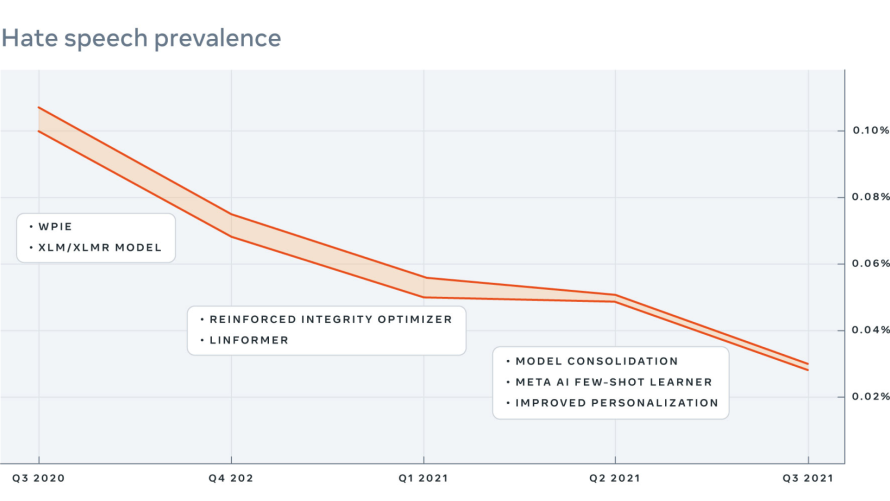
\includegraphics[width=.8\textwidth]{images/fsl_chart.png}
  \caption{Comparison between new few shot learner and
    older models, source: \cite{site:AIart}}
  \label{fig:aichart}
\end{figure}

%% FRAMEOWORK
% framework comunque � il business model canvas.
\subsection{Analytical framework}\label{sub:analytical}
To analyze the business model of Facebook we will use the business
model canvas. This tool, originally developed by Alexander Osterwalder
in \cite{art:osterwalder2010business} identifies nine components of a
business model. These nine components are key partners, key
activities, key resources, value proposition, customer relationships,
channels, customer segments, cost structure and revenue stream. More
in detail:
\begin{description}
\item[key partners] the main organizations or individuals the company
  is interacting with;
\item[key activities] the activities that the value proposition, the
  distribution channels, the customer relationships or the revenue
  stream require;
\item[key resources] similarly to key activities are the resources
  required by the value proposition, the distribution channels, the
  customer relationships or the revenue stream;
\item[value propositions] these are the main focus of the canvas,
  analyzes what is the value that the company delivers to customers,
  which are the customer's problems that the company is helping to
  solve and which customer's need is the organization satisfying;
\item[customer relationships] are what type of relationships does each
  customersegment expect to enstablish and mantain with the company
  and how costly are they;
\item[channels] the channels trough wich the customers want to be
  reached, ho wth eocmpany is actually reaching them, how the channels
  are integrated, which kind of channel works the best, the costs of
  each channel and how th company is integrating these channels in
  customer's routines
\item[customer segments] who actually are the customers;
\item[cost structure] This is actually one of the main two point of
  the canvas. Identify which are the most important inherit costs of
  the business model, based on the factors we previously described;
\item[revenue streams] this is the other main point of the
  canvas. This section analyzes what the customers are actually
  willing to pay for, what are they currently paying for, how, and how
  would they prefer to pay, laong with how each revenue stream
  contributes to the total revenue stream of the company.
\end{description}

\begin{figure}
  \centering
  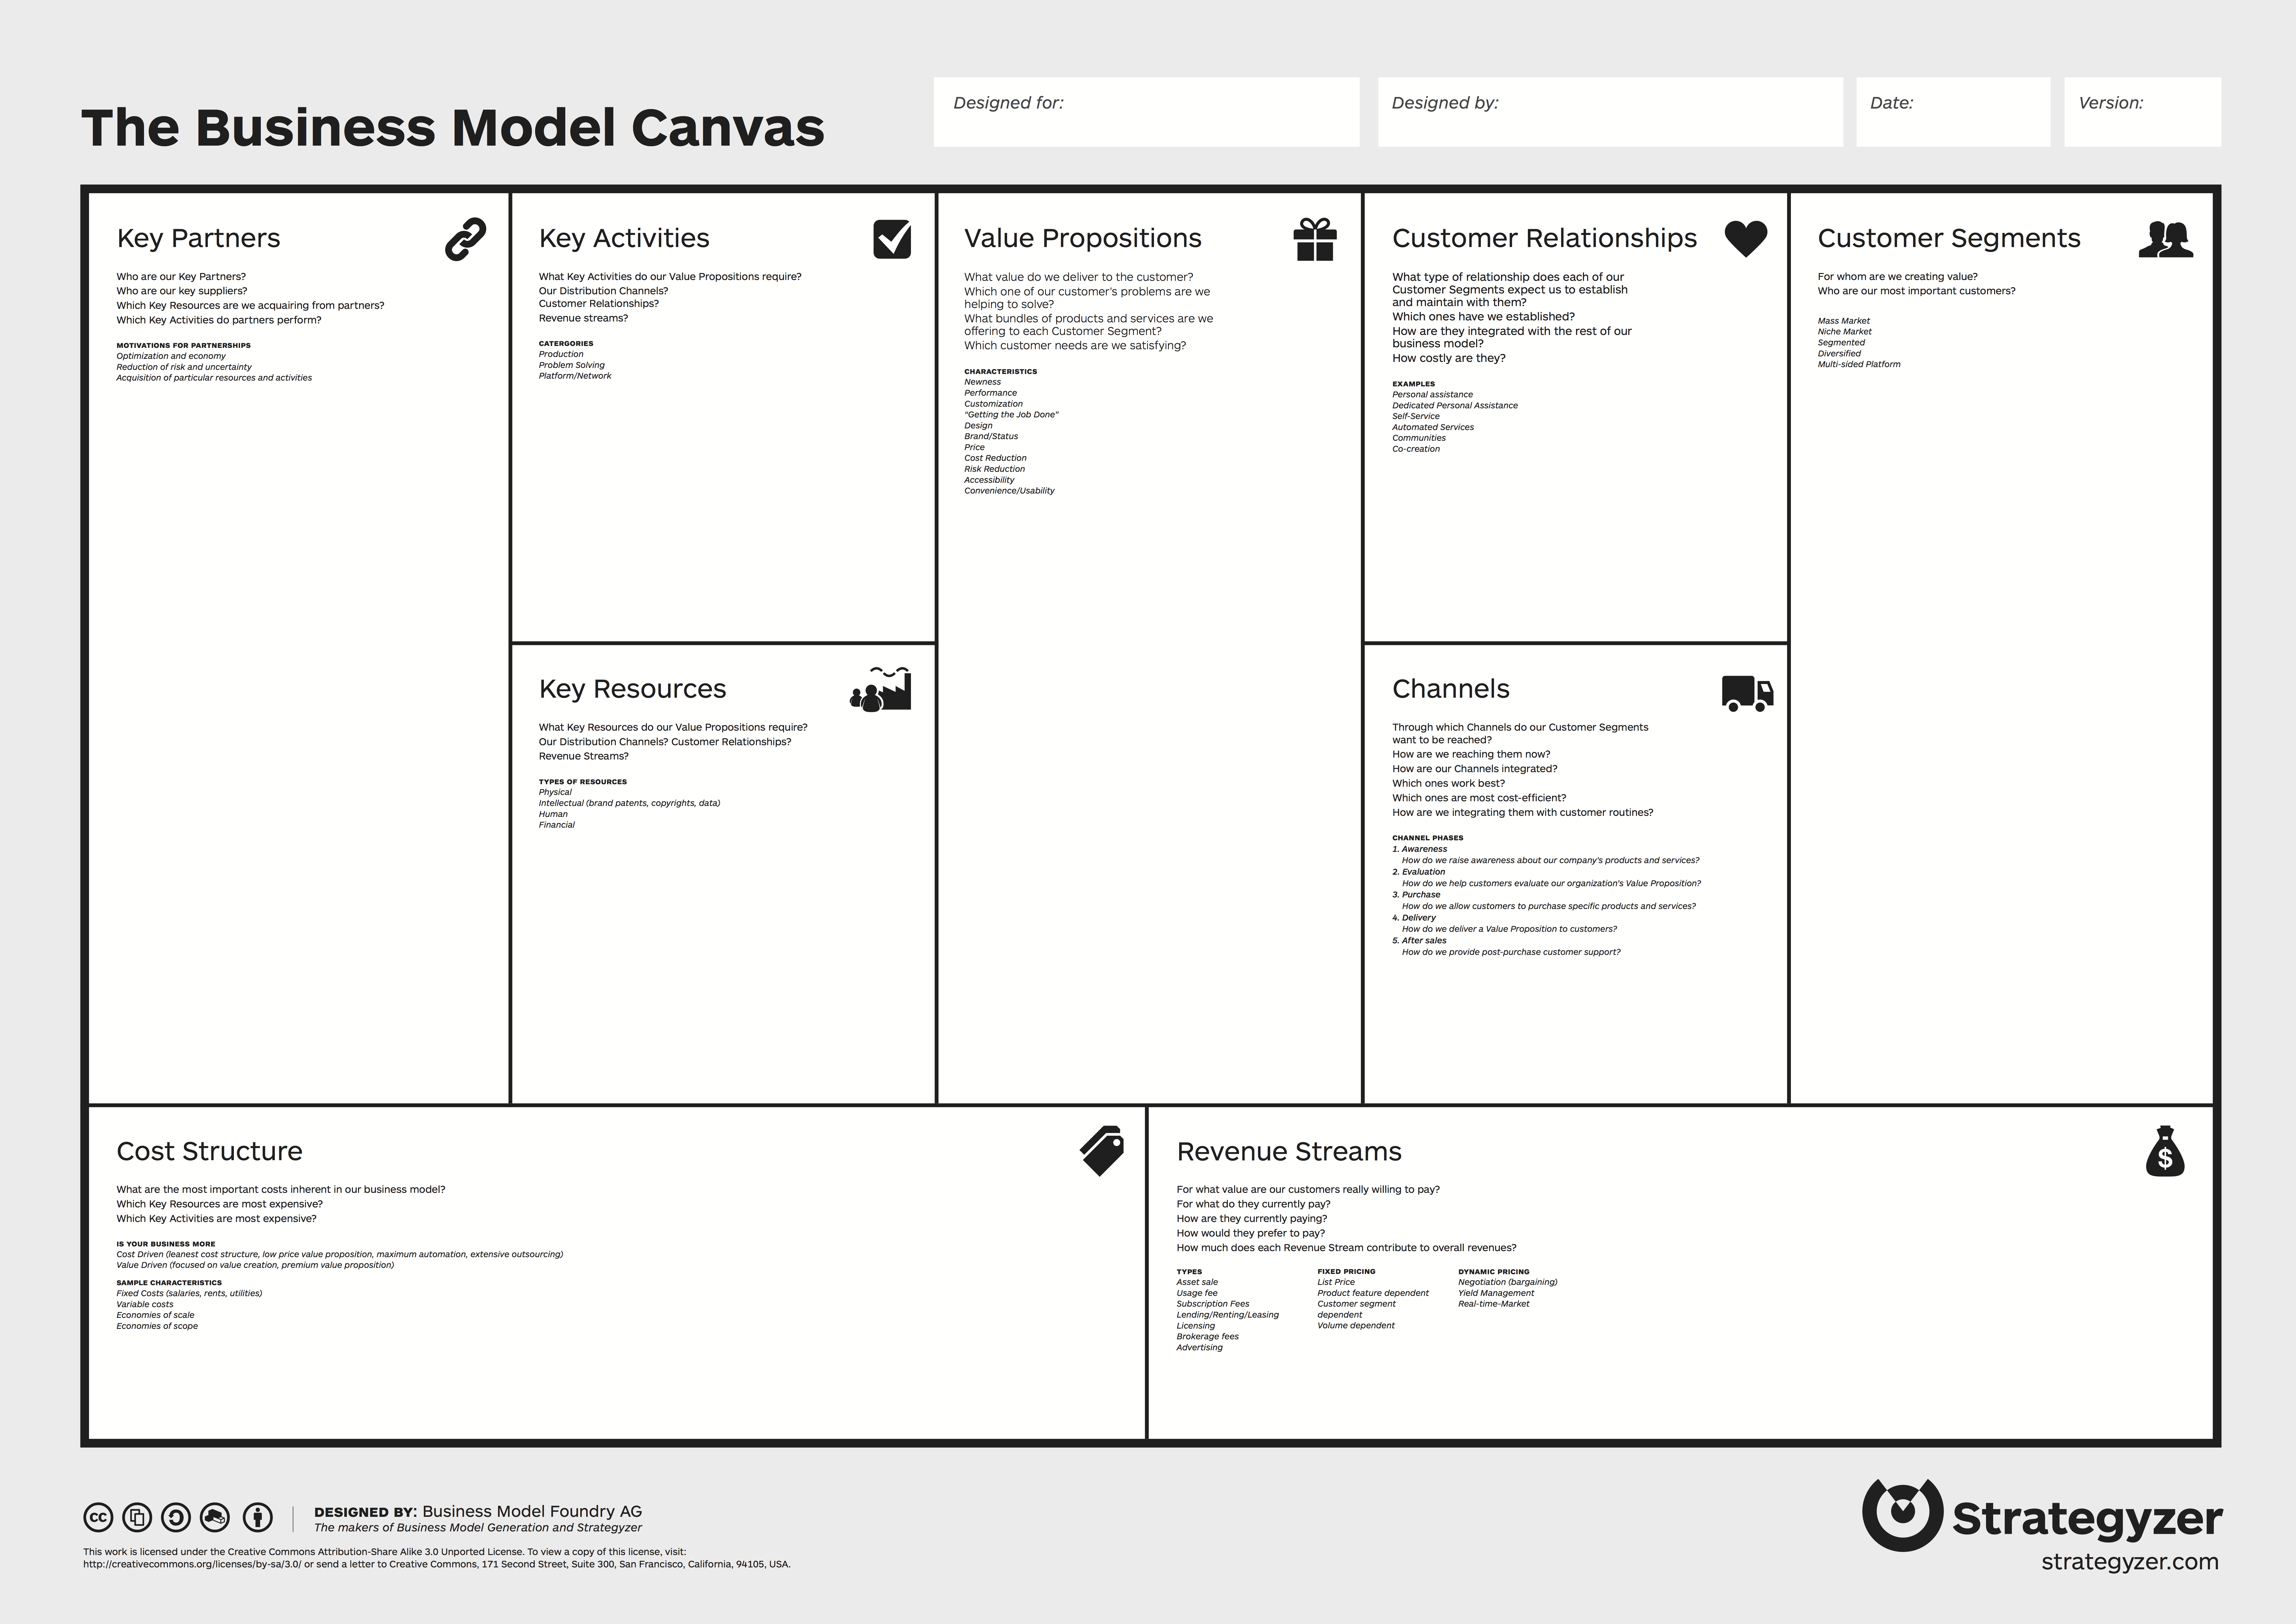
\includegraphics[width=.8\textwidth]{images/Business_Model_Canvas.png}
  \caption{Business model canvas template, source:
    \cite{site:bmcanvas}}
  \label{fig:bmcanvas}
\end{figure}

The figure \ref{fig:bmcanvas} shows a template for this business model
canvas. This tool is particularly useful to understand how this
innovation affects the company in the supply chain to its customers,
and to analyze the impact it can have on keeping a sense of trust
between the customers and the company.
